 \documentclass[linenumbers,twocolumn]{aastex631}

\usepackage{longtable}
\usepackage[flushleft]{threeparttable}
\usepackage{tabularx}
\usepackage{multirow}
\usepackage{graphicx}
\usepackage{amsmath,amssymb}
\usepackage{color}
\usepackage{units}
\usepackage{epstopdf}
\usepackage{hyperref}
\usepackage{multirow}
\usepackage{url}
\usepackage{subfigure}
\usepackage{rotating}
\usepackage{enumitem}\setlist[description]{font=\textendash\enskip\scshape\bfseries}
% \usepackage{lineno}

\usepackage[colorinlistoftodos]{todonotes}

% \linenumbers

%\usepackage[doublespacing]{setspace}

\newcommand{\braket}[2]{\left\langle#1\, |\,#2\,\right\rangle}  %  < #1 | #2 >
\newcommand{\expec}[1]{\langle#1\rangle}  %  < #1 >
\newcommand{\drm}{{\rm d}}
\newcommand{\irm}{{\rm i}}
\newcommand{\beq}{\begin{equation}}
\newcommand{\eeq}{\end{equation}}
\newcommand{\bdm}{\begin{displaymath}}
\newcommand{\edm}{\end{displaymath}}
\newcommand{\T}[1]{\tilde{#1}}
\newcommand{\wT}[1]{\widetilde{#1}}
\newcommand{\Cdot}{\!\cdot\!}
\newcommand{\SNR}{\textnormal{SNR}}
\newcommand{\rednote}[1]{{\color{red} (#1)}}
\definecolor{Gray}{gray}{0.9}
\definecolor{orange}{rgb}{0.9,0.5,0}
\newcommand{\td}[1]{{\textcolor{orange}{\texttt{TD: #1}} }}
\newcommand{\zd}[1]{{\textcolor{purple}{\texttt{ZD: #1}}}}
\newcommand{\muj}[1]{{\textcolor{red}{\texttt{MU: #1}} }}
\newcommand{\sa}[1]{{\textcolor{blue}{\texttt{SA: #1}}}}
\newcommand{\ztfrest}{\text{ZTFReST }}
\newcommand{\ttt}[1]{\texttt{#1}}
\newcommand{\jp}[1]{{\textcolor{blue}{#1}}}

\newcommand{\nmma}{\text{NMMA }}

\newcommand{\ztfink}[1]{ZTF-Fink}
\newcommand{\fink}{{\sc Fink}}

% Load results from results.tex so these can be updated automatically
% This file was automatically generated; edits will be overwritten!
\newcommand{\boomthroughputfactor}{6}
\newcommand{\kakfaingestratembps}{XXXXX}
\newcommand{\kakfaingestfactor}{XXXXX}


%\graphicspath{{./plots/}}

\begin{document}

\title{A real-time, multi-survey, optical alert system broker operating at scale}

% Abstract of the paper
\begin{abstract}
With the arrival of ever higher throughput wide-field surveys and a multitude of multi-messenger and multi-wavelength instruments to complement them, software capable of harnessing these associated data streams is urgently required. To meet these needs, a number of community supported \emph{alert brokers} have been built, currently focused on processing of Zwicky Transient Facility (ZTF; $\sim 10^5$--$10^6$ alerts per night) with an eye towards Vera C. Rubin Observatory's Legacy Survey of Space and Time (LSST; $\sim 2 \times 10^7$ alerts per night). Building upon the legacy of a successful system that ran in production for ZTF for the first seven years of its operation, we introduce \texttt{BOOM} (Burst \& Outburst Observations Monitory), an analysis framework focused on real-time, joint brokering of these alert streams.
Harnessing the performance of a \texttt{Rust}-based software stack relying on a non-relational (NoSQL) \texttt{MongoDB} database combined with a \texttt{Redis}/\texttt{Valkey} in-memory processing queue and a \texttt{Kafka} cluster for message sharing, we demonstrate feature parity with the existing ZTF system with a throughput $\sim \boomthroughputfactor \times$ higher.
We describe the workflow that enables the real-time processing, as well as results with custom filters we have built to demonstrate the system's capabilities.
We further outline the development plan for \texttt{BABAMUL}, the public version of \texttt{BOOM} processing LSST alerts.
Finally, we outline the development plans for \texttt{BOOM} as we begin the LSST era.
\end{abstract}

%%%%%%%%%%%%%%%%%%%%%%%%%%%%%%%%%%%%%%%%%%%%%%%%%%

\listoftodos

%%%%%%%%%%%%%%%%% BODY OF PAPER %%%%%%%%%%%%%%%%%%

\section{Introduction}

Modern optical surveys now scan the entire sky daily, reaching depths that allow detection of both distant, bright objects and nearby, faint ones. This capability enables the discovery of rare phenomena, a census of the variable sky, and tests of fundamental physics at energy scales far beyond those of terrestrial accelerators. However, fully exploiting these opportunities is currently constrained as much by software and data processing methods as by available instrumentation.
The upcoming Vera C. Rubin Observatory's Legacy Survey of Space and Time (LSST) exemplifies the scale of future transient discovery \citep{Ivezic2019}. LSST will scan large swaths of the sky to unprecedented depths. Each potential discovery will be immediately broadcast to the community as an alert, not to the entire community but to a set of pre-selected alert brokers, tasked with redistributing the data stream to the wider community, while providing easy-to-use tools to search for and visualize candidates of specific astronomical objects.
For comparison, the Zwicky Transient Facility (ZTF) \citep{Bellm:19:ZTFScheduler,Graham2018,DeSm2018,Masci2019}, the current survey that the community most commonly uses for transient follow-up, produces $\sim 10^5$--$10^6$ alerts per night, while LSST will be more than an order of magnitude larger ($\sim 2 \times 10^7$).

Real-time processing and rapid follow-up of this alert stream is critical for many science cases, with brokering software needing to keep up with the rate of alerts while maintaining or increasing the number of features it aims to offer to the end user. The alerts emitted by these large surveys include a variety of transient phenomena, including very young Type Ia supernovae (SN\,Ia) with either an early ``flash'' or ``bump'' in their light curves well before the epoch of maximum light (e.g., iPTF14atg; \cite{cao_strong_2015}, SN2017cbv; \cite{Hosseinzadeh_2017} and SN2019yvq; \cite{Miller_2020}), luminous fast blue optical transients (LFBOTs) \cite{PrMa2018,Perley2019,HoGo2019,HoPe2020,Perley_2021}, with optical and (sometimes) copious X-ray emission evolving on short timescales, $\gamma$-ray burst afterglows \cite{NyFr2009,GeMe2012} from either collapsars or neutron star mergers, kilonovae associated with binary neutron star mergers \citep{AbEA2017b} such as AT2017gfo \citep{CoFo2017,SmCh2017,AbEA2017f}, and jetted tidal disruption events whose accretion leads to the launch of a relativistic jet \citep{Bloom2011Sci,Andreoni_2022}, amongst many other science cases. These young and/or fast transient science cases are bolstered by the rise of instruments in other messengers, e.g., Advanced LIGO \citep{aLIGO} and Advanced Virgo \citep{adVirgo} for gravitational waves, e.g., IceCube \citep{AaAc2017} for neutrinos, or other wavelengths,  the {\it Neil Gehrels Swift Observatory} mission \citep{GeCh2004}, Fermi's Gamma-ray Burst Monitor (Fermi-GBM) \citep{MeLi2009}, the Space-based multi-band astronomical Variable Objects Monitor (SVOM), and Einstein Probe \citep{Yuan_2022} for $\gamma$-rays and X-rays.

There is a large software ecosystem enabling time-domain astronomy.
For example, the General Coordinates Network (GCN; \citealt{SiRa2023}) and the Scalable Cyberinfrastructure to support Multi-Messenger Astrophysics\footnote{\url{https://scimma.org/}} (SCiMMA) project are platforms where multi-messenger instruments share real-time alerts with the community that can then be either followed-up directly or cross-matched with alert streams.
Depending on the type of transient, it is common for identified transient objects to be shared with the community on the Transient Name Server\footnote{\url{https://www.wis-tns.org/}} (TNS) or the Minor Planet Center\footnote{\url{https://minorplanetcenter.net/}} (MPC).
These streams are ingested by Target and Observation Managers (TOM), otherwise known as ``marshals,'' which enable coordinated follow-up efforts; examples include \texttt{YSE-PZ} \citep{CoJo2023}, TOM Toolkit \citep{StBo2018}, and \texttt{SkyPortal} \citep{WaCr2019,Coughlin_2023}.

Feeding these Marshals are the ``enriched'' alert streams from the brokers, which include, among others, ALeRCE \citep{FoCa2021}, AMPEL \citep{Nordin:2019kxt}, ANTARES \citep{MaSt2021}, Fink \citep{MoPe2020}, Lasair \citep{SmWi2019}, Pitt-Google, and \texttt{BABAMUL} (the plans for which we will discuss further below). These brokers filter the optical alert streams to identify targets of interest. For surveys like ZTF and LSST, alerts are produced when a significant ($< 5 \sigma$) residual flux is detected from a point source in a subtracted image, and are distributed via Kafka\footnote{https://kafka.apache.org} in Apache avro format. While each survey provides a different set of data -- and therefore uses a different schema to serialize it -- they all include key properties such as:
\begin{itemize}
\item Position and brightness of the current detection
\item Ancillary detection data and higher-level derived values, including real--bogus scores, which helps distinguish real transients from image artifacts.
\item The associated triplet of science, reference, and subtraction images
\item Time-series information about past alert-based detections, non-detections, and forced photometry
\item Higher-level metadata about a known astronomical object at the location of the detection (to within some positional uncertainty).
\end{itemize}

To identify the most interesting objects for particular science cases, brokers can cross-match alerts against static catalogs (e.g., Gaia DR3, \cite{Gaia2023}; PanSTARRs DR1, \cite{ChMa2016}; milliquas, \cite{Flesch_2023}; NED LVS, \cite{Cook_2023}) and look for specific properties using machine learning classification pipelines (e.g., AstroM3, \cite{rizhko2024astrom}; BTSbot, \cite{Rehemtulla+2024}; ACAI, \cite{duev2021phenomenologicalclassificationzwickytransient}; Maven, \cite{zhang2024mavenmultimodalfoundationmodel}). All brokers provide their own filtering system which make use of the ``enriched'' alert data to identify objects of interest for specific science cases. Depending on the broker, the filters can be from a standard set defined based on community feedback or customized by the user. Also, they may run in real-time as alerts are coming in, or anytime after the alert data is processed to perform archival searches. So far, alert brokers have been providing these services predominantly on the ZTF alert stream. However, now that a number of surveys providing real-time alert streams will overlap in space and time, we -- as a community -- have an opportunity to enrich each survey with the data products from the others.

Specifically, to supplement LSST's alert stream, a variety of other optical systems such as the La Silla Schmidt Southern Survey (LS4; \citealt{miller2025lasillaschmidtsouthern}) and ZTF will be trailing the LSST footprint nightly. To maximize the science synergies enabled by these coordinated observations, brokers will need to perform joint filtering on these alert streams. This will be essential to, for example, readily identify fast transients within these streams, as the relatively slow cadence of LSST will otherwise make it difficult to identify such phenomena, and the limited depth from other optical surveys makes it difficult to precisely constrain their rate of evolution.

It is with these considerations in mind that we present \texttt{BOOM}, a broker that builds upon our experience with \texttt{Kowalski}\footnote{\url{https://github.com/skyportal/Kowalski}}, an open-source, multi-survey data archive and alert broker \citep{DuMa2019} that has run in production for the ZTF collaboration for the last seven years.
In this paper, we will describe several important developments and design choices with \texttt{BOOM} that ready it for the upcoming LSST era.
Although this paper focuses mainly on the design and conceptual framework of \texttt{BOOM}, we encourage the interested reader to also see the documentation in the repository\footnote{https://github.com/boom-astro/boom} and to explore the repository alongside this text.
As an example of important design choices, due to the fact that multiple observatories will observe the LSST footprint, \texttt{BOOM} has, as a top priority, the ability to jointly filter on multiple alert streams, a relatively unique capability in the broker community.
Furthermore, one of the main differences between \texttt{BOOM} and \texttt{Kowalski}---and most other alert brokers---was moving away from Python and instead writing the project in Rust, a compiled programming language with performance characteristics that make it much better suited to attaining a high throughput of alerts at scale. Processing additional alert streams in parallel already increases the data volume by at least an order of magnitude, and jointly filtering on multiple streams at once requires even more computation, as every alert packet needs to be cross-matched with all other overlapping surveys' alert streams.
While this has the downside of making contributions from astronomers, who typically write in Python, more challenging, our experience running \texttt{Kowalski} in production has shown us that requiring any computer science knowledge to make use of an alert broker (at least, for non-complex tasks) will significantly limit its use, regardless of complexity. Below, we will describe the filtering framework we have built to ameliorate this challenge, where the user is provided with a no-code alternative to write complex queries.

In this paper, we describe the components built within \texttt{BOOM}, focusing on design choices useful in preparation for LSST data scales.
We describe \texttt{BOOM}'s key features in Sec.~\ref{sec:pipeline}.
We demonstrate some of \texttt{BOOM}'s capabilities, including throughput measurements, in Sec.~\ref{sec:science}.
We describe the future of \texttt{BOOM} and how we envision its role in the community in Sec.~\ref{sec:conclusion}.

\section{\texttt{BOOM} Framework}
\label{sec:pipeline}

\begin{figure*}[t]
    \centering
    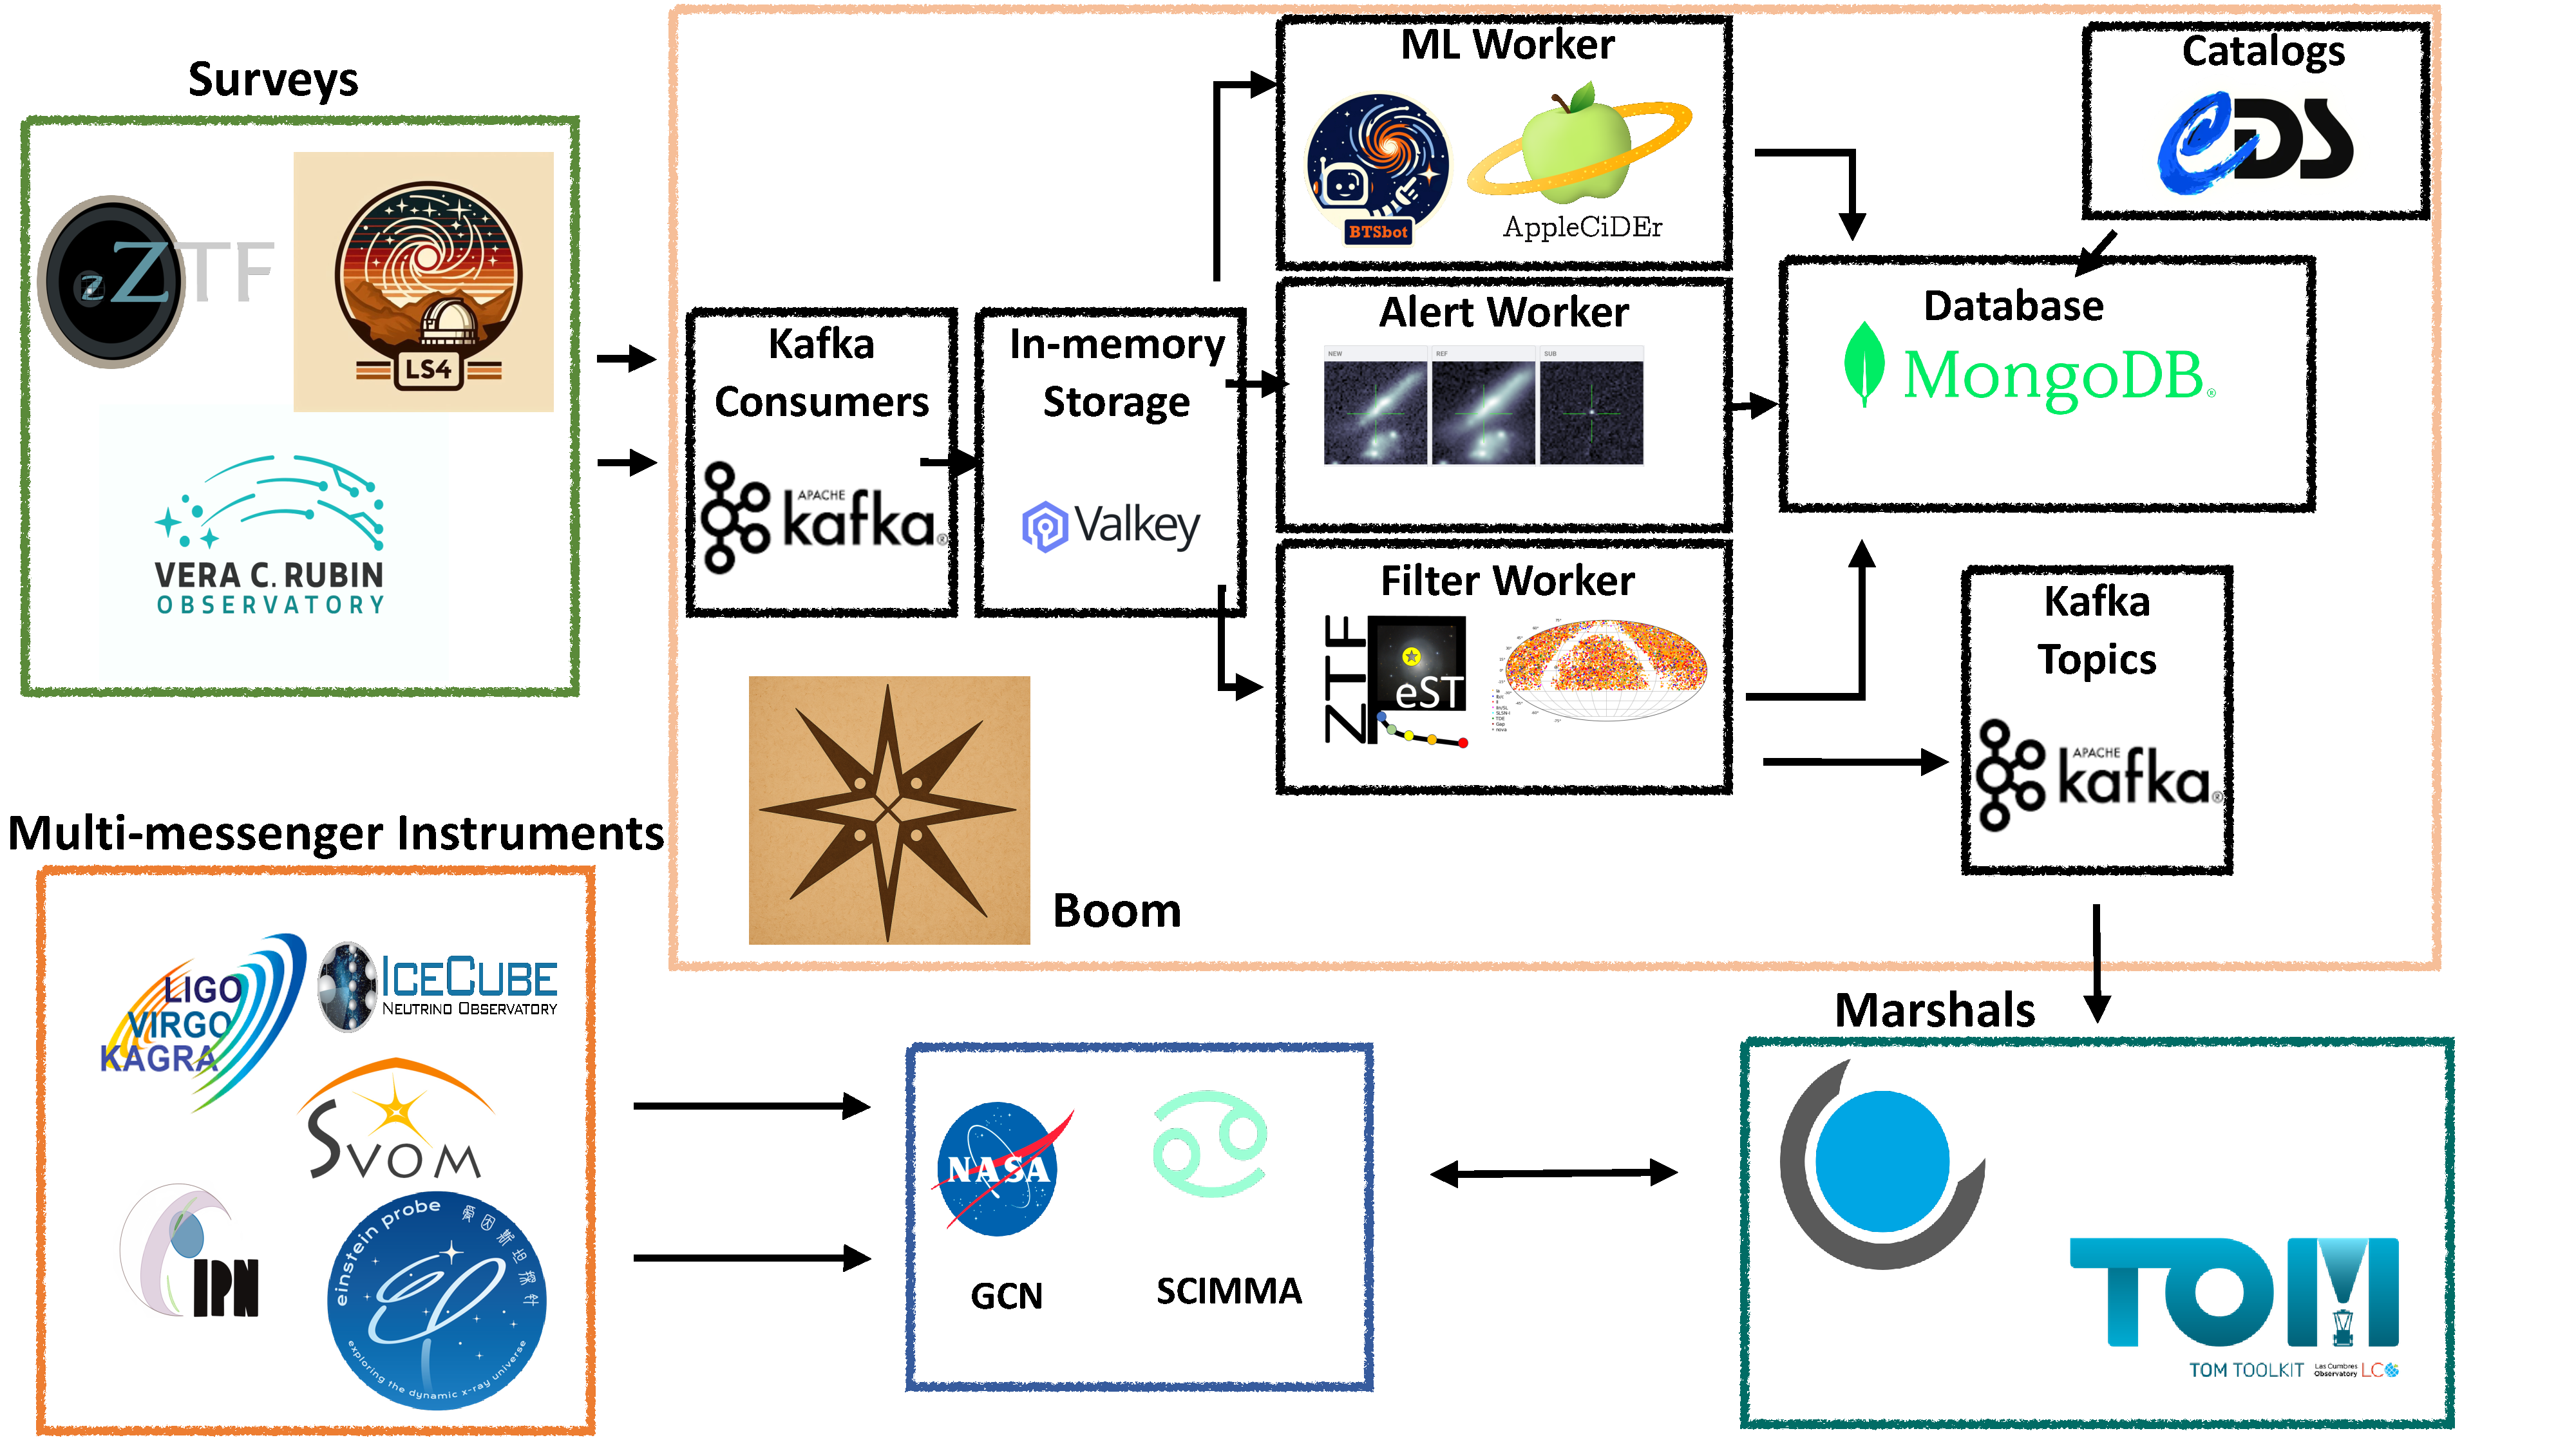
\includegraphics[width=6.5in]{figures/workflow.pdf}
    \caption{Flowchart for BOOM.}
    \label{fig:flowchart}
\end{figure*}

In the following subsections, we present the key design features and implemented capabilities within \texttt{BOOM}.
\texttt{BOOM} is designed for full parallelization. The database and alert processors all scale horizontally, allowing additional workers to be added at any stage to accommodate changes in workload. Alerts can be processed in any order, meaning they do not need to follow a strict time sequence.
\texttt{BOOM} operates with workers, separating the machine learning, cross-matching, filtering, ingestion, etc. into different processes. Each of these workers are described herein.

\subsection{Input/Output through \texttt{Apache Kafka}}

\texttt{Apache Kafka} has become the gold standard for astronomical alert brokering due to its scalability, fault tolerance, and capacity to handle large data volumes for a wide variety of production-grade software, in academia and industry. Optical alerts from surveys like ZTF and LSST are transmitted as Avro packets\footnote{\url{https://avro.apache.org}} over Kafka, which means that the ability to feed from \texttt{Kafka} topics, which represent one data stream that a client can read from, is absolutely required by any alert brokering software. Its ecosystem of libraries available for all major programming languages makes it extremely easy to the client to develop pipeline around it. For these reasons, also adopting \texttt{Kafka} as our downstream message sharing system ensures compatibility with existing downstream services, which are designed to consume alerts from \texttt{Kafka}. For each survey supported by our software, an associated \texttt{Kafka} consumer has been developed to feed from the \texttt{avro}-formatted alerts. The consumers take advantage of \texttt{Kafka}'s partitioning feature (where one topic is broken down in N partitions that a client can read from independently, with multiple processes) to process any given survey's alert stream(s) in parallel, maximizing the input rate.

% To evaluate scalability, we tested various Kafka producer configurations simulating an LSST-like data stream. Our results show that our Kafka cluster can ingest all topics at \rednote{\kakfaingestratembps} MB/s, approximately \rednote{\kakfaingestfactor} times faster than the anticipated LSST average alert production rate.

\todo[inline]{
    maybe the section under that comment should move elsewhere, or be in some
    info-card like we did in the NSF WOU ZTF+LSST proposal, to highlight the
    capabilities of Rust and its relevance for this project?
}

Instead of implementing an alert consumer software for every survey, we heavily rely on \texttt{rust}'s \texttt{Trait} system. \texttt{Trait} lets a developer define a blueprint for \texttt{Struct}s, which are \texttt{rust}'s data structure equivalent to Python classes. Thereafter, functions can be written to not take specific \texttt{Struct}s as input, but anything that implements one or more \texttt{Trait}s. For example, we define the \texttt{AlertConsumer} trait with a method definition called \texttt{consume} (responsible for reading from \texttt{Kafka} with survey-specific parameters). Then, the main function responsible for reading from \texttt{Kafka} specifies that it takes any \texttt{Struct} that implements the \texttt{AlertConsumer} trait as input. This ensures type-safety across a codebase, while minimizing duplication and without sacrificing performance. Also, when multiple \texttt{Struct}s implementing the same \texttt{Trait} have an identical implementation for a function, that function can simply be defined and implemented in the trait itself, to avoid re-defining it in any of the \texttt{Struct}s.
This \texttt{Trait}, \texttt{Struct}s, and generic functions pattern is repeated throughout the BOOM codebase, where all alert processors that share common operations between at least two surveys can be deduplicated. By ensuring that little to no code is duplicated from one survey to another, we can ensure BOOM's scability as more surveys are supported in the future.

\subsection{Job scheduling with \texttt{Valkey}}

Whereas \texttt{Kafka} shines when it comes to reliably sharing
messages at scale across the web,
it is not the most performant solution for inter-process communication,
as topics are stored on disk,
which results in a throughput limited by the host's I/O capabilities.
Instead, we opted for \texttt{Valkey},
a high-performance in-memory datastore backed by the Linux Foundation.
\texttt{Valkey} can be used for a variety of workflows,
including caching and message queues.
Unlike \texttt{Kafka},
all data stored with \texttt{Valkey} lives in RAM,
ensuring a much higher throughout than physically possible on HDDs or SSDs.
Once data is read from the various survey's \texttt{Kafka} topics,
\texttt{BOOM}'s \texttt{Kafka} consumer stores alerts to be processed in
a \texttt{Valkey} list;
this is a simple array from which processes on the same machine or network
can read from, one element at a time or in batches.
When read from a list, messages are removed from it,
and therefore only are retrieved by one process at a time.
This is precisely what we need for \texttt{BOOM},
where alert processing is not performed by one but many processes,
to parallelize over the streams.
Also, \texttt{BOOM} does not rely on one process to ingest, enrich,
and filter a stream one alert at a time,
but instead is composed of dedicated processes
for each of these processing steps;
\rednote{this approach and technical choice is detailed in section X}.
\todo[inline]{Fix reference for section.}
There, \texttt{Valkey} is used to communicate data between various
processes with high-throughput.
However, memory usage becomes a concern when relying heavily on
in-memory storage technologies.
With this in mind, \texttt{BOOM} sets limits on how many
\texttt{Apache} Avro alert packets are stored in memory at once.
Other message queues used in \texttt{BOOM} only share a minimal amount of
information (mostly pointers to database documents,
and unique identifiers of alert packets),
and do not have a noticeable memory impact.

\subsection{Spatial query-ready database with \texttt{MongoDB}}

\texttt{MongoDB} has proven to be a highly effective choice for alert brokering, as demonstrated by its successful implementation in \texttt{Kowalski}. Its cross-language support, flexibility, and powerful query language make it well-suited for building complex filtering pipelines for transient alerts. Namely, the \texttt{aggregation pipeline} feature has allowed us to define not only complex queries but also a pipeline of queries with multiple stages, such as a cycle of filtering (\$match stage), computing (\$project, \$addField, \$lookup ... stages) steps, well-suited to implement astronomical alert filtering pipelines. \texttt{MongoDB} offers both performance and scalability, essential for handling large data volumes efficiently. While \texttt{PostgreSQL} was a potential alternative, it would have required schema enforcement, limiting adaptability in an alert stream where fields can vary significantly or evolve in time. Moreover, \texttt{PostgreSQL} would have necessitated database migrations whenever a new astronomical catalog was integrated for crossmatching, and does not offer native support for common spatial queries (e.g. cone searches). By contrast, \texttt{MongoDB}'s schema-free design allows \texttt{BOOM} to dynamically accommodate new data sources without modifying the database structure, and natively supports \texttt{GeoJSON} indexes for fast spatial queries, such as cone-searches or nearest neighbour searches without any client-side implementation or extensions required. Just like \texttt{Kowalski}, \texttt{BOOM} relies very heavily on \texttt{MongoDB}'s support for cone-searches of alert streams with archival/static catalogs, and other alert streams.

\todo[inline]{
    This section deserves more work,
    I think we could maybe give a little more technical details about
    what things look like, and maybe that's also the right place to describe
    how each survey has 3 catalogs: one for individual candidates/alerts,
    one for images/cutouts associated to these alerts,
    and one for astronomical objects.
}

\subsection{Parallelized and Distributed Alerts Processing}

It had become clear with \texttt{Kowalski} that making one process responsible
for processing one alert at a time in its entirety
(i.e. ingestion, enrichment,
and filtering) does not allow us to scale optimally.
When one of the processing steps becomes a bottleneck,
the only solution with a single worker approach is
to make more copies of the same worker,
rather than only scale the processing
step that requires more resources to keep up with the expected throughput.
For example,
with the advances of machine learning techniques yielding ever larger
and complex models,
adding more models to run on an alert stream requires more
compute time not for every step of the processing but only to run these
additional models.
Therefore, the ability to only scale processes responsible of
running models without also allocating resources to other processing steps,
which do not need them, is much more effective and scalable.
Next, we will describe
how the alert processing steps have been split in multiple ``workers:''

\todo[inline]{
    PB: I'm still struggling to understand how splitting a serial pipeline
    into multiple queues increases throughput without running on a cluster
    with heterogeneous compute nodes, for example.
    Maybe a diagram would be helpful here.
    It seems like batching, not multiple queues,
    would produce the biggest performance gain.
    Or, doing ML inference for all models in parallel,
    since that's the only thing we can do concurrently to a given alert.
    I started a notebook in the \texttt{boom-paper} repo on GitHub
    to simulate the different architectures using SimPy
    in case we want some evidence to back up this relatively strong statement:
    ``much more effective and scalable''.
}

\subsubsection{Alert Ingestion Worker}

\texttt{BOOM}'s first worker type is the \texttt{Alert Ingestion} worker. It feeds from the \texttt{Valkey} queue that has been populated with \texttt{Apache} Avro alert packets by the consumer(s), and its main role is to ingest xmatch-enriched reformatted alerts to the \texttt{MongoDB} collections of a given survey. It processes one alert packet at a time (multiple workers of this type are spawned to handle the load), going through the following streams:
\begin{itemize}
\item Read the \texttt{Apache} Avro byte data to deserialize into \texttt{rust} \texttt{Struct}s matching the schema provided by the survey emitting the alerts. Here, we really heavily on the \texttt{serde} and \texttt{apache-avro} rust structs; the former also allows us to customize the deserialization logic to modify the alert data's schema of each survey, in an effort to reduce some of the differences between different surveys' schemas, and to address some of their inefficiencies.
\item We separate the candidate metadata about the current detection, candidate identifier (referred to as candid, the unique identifier of the candidate), and object identifier (objectId, the unique identifier of the associated object) from its cutout images and time-series.
\item The candidate, its identifier and associated object's identifier are stored in the alert collection (indexed by candidate id).
\item The science, reference, difference cutout images are stored in the cutout collection (also indexed by candidate id).
\item For new objects -- identified as the objects for which no entry indexes on the associated objectId is found in the object-level table -- we cross-match the candidate's position with a number of static/archival catalogs. Since a new objectId is generated when we receive the first alert at a given right ascension and declination ($\pm$ some uncertainty that varies based on a survey's hardware and pipeline), and thereafter alerts at the same position are associated to the same objectId, cross-matches with static catalogs only need to happen once for a given objectId. As the position and catalog are immutable, so are the results of a cross-match. Cross-matches happen directly in the database using its native support for cone searches, using a GeoJSON index. Here, the radius used is the maximum between the positional uncertainty of the alert survey and the positional uncertainty of the instrument that was used to build the static catalog.
\item Similarly, we cross-match every alert with the object collection of other surveys supported by \texttt{BOOM}. While the position is still immutable for a given objectId, here the catalogs we cross-match against are dynamic, populated with new objects as the surveys generate alerts at new positions. The cross-match radius is defined as the maximum positional uncertainty between two surveys being cross-matched.
\item Last but not least, we either create or update the object collection. New objects get a new entry in the object collection indexed on their objectId, containing the time-series (previous candidates, non-detections, and forced-photometry), and cross-matches with archival and static catalogs. For existing objects, the various time-series have new elements appended, and cross-matches with dynamic catalogs are updated.
\end{itemize}

Once an alert has been ingested, its candid is pushed to another \texttt{Valkey} queue for the next worker to read from. Surveys that can be enriched with machine learning scores have their candIds sent to a queue that will be read by the \texttt{ML worker} (see Sec.~\ref{sec:ML}), otherwise these are directly sent to the \texttt{Filter worker} (see Sec.~\ref{sec:filter}).

\subsubsection{Machine Learning Worker}
\label{sec:ML}

While there is no obvious advantage to ingesting alerts in bulk -- other than reducing round trips to the database, which we will explore in future iterations of \texttt{BOOM} if the alert ingestion becomes a bottleneck -- there is a clear advantage to running machine learning models over batches of inputs, as these can easily be parallelized by the various Machine Learning frameworks available to us, using hardware accelerators (e.g. GPUs, TPUs). So, a Machine Learning worker will not read only one candid from \texttt{Valkey} but will a batch with a set maximum size (e.g. 1000 at a time, if less than 1000 alerts are queueing for inference, instead of blocking until 1000 are available the machine learning worker will simply read as many candids as available). Once the candId are retrieved, we use an aggregation pipeline to retrieve the candidate, associated images, and full light curve(s) from the database. The alert data is then converted into the expected format for each machine learning model \texttt{BOOM} supports (if multiple models expect the same input data, features are only prepared once to avoid duplicating work). At this time, \texttt{BOOM} runs all 5 ACAI classifiers \citep{Duev+2021}, and BTSbot \citep{Rehemtulla+2024}. These models have successfully been used in Kowalski for a number of programs, including fully-automated follow-up programs.
While most popular machine learning frameworks have been designed in Python and therefore not usable as-is in Rust or other languages, there are a number of solutions to port \texttt{Python}-trained models over to a \texttt{rust}-based pipeline. One can choose between:
\begin{itemize}
\item If the Python ML framework used is built around a C-based low-level library, bindings are often available to run the same models in Rust (e.g. Tensorflow, Pytorch). However, these proved to lack community support as well as documentation, and to require a number of additional system dependencies, making it an unsustainable approach.
\item Since we are relying on a ``compartimentalized'' architecture with a worker type dedicated to machine learning that interacts with \texttt{redis} and \texttt{mongodb}, both of which are well supported in \texttt{Python}, one could simply implement this worker directly in \texttt{Python}. In fact, \texttt{BOOM}'s architecture has been designed to maximize flexibility and inter-operability between languages, and was initially designed with a \texttt{Python}-based machine learning worker. However, we later decided to opt for a fully \texttt{rust}-based approach as we successfully converted \texttt{Kowalski}'s \texttt{Python}-trained model to a format suitable for running directly in \texttt{rust} (described below).
\item The \texttt{pyo3} crate allows for seemless integration of Python code in a \texttt{rust} runtime. Using this package, a developer can directly run Python code within a rust program. However, this did not prove to yield a significance performance improvement compared to the complexity added to the software. Also, a lack of documentation and community-backed examples applied to machine learning with \texttt{pyo3} steered us away from this option.
\item Last but not least, most standard machine learning implementations, regardless of the framework used, can be converted to a framework and language agnostic format called \texttt{ONNX} (Open Neural Network eXchange) \footnote{\url{https://onnx.ai/}}. \texttt{ONNX} is an open-source format that defines a set of common operators, to represent models trained in most ML frameworks in a graph-like format. Community-driven Python packages for both PyTorch and Tensorflow allow users to convert their trained model to the \texttt{ONNX} format, which can then be loaded in all languages for which an \texttt{ONNX} runtime has been implemented. In Rust, the \texttt{ort} crate (https://ort.pyke.io/) allows us to load any \texttt{ONNX} model, while enabling graph representation optimization; \texttt{ONNX}'s graph optimizer is able to remove unnecessary, redudant, or suboptimal operators/nodes generated when converting models to this format, often allowing for higher levels of optimizations than achievable when running inference in the original framework used to train the model). It also allows for hardware acceleration (\texttt{ort} supports CPU, GPU, and TPU as well as a variety of backends well-suited for specific hardware, e.g. NVIDIA's \texttt{CUDA} or Apple's \texttt{CoreML}).
\end{itemize}

After experimenting with all 4 approaches, integrating \texttt{ort} in a \texttt{rust}-based program to run \texttt{Python}-trained models converted to \texttt{ONNX} yielded the best ``performance vs. complexity'' ratio. So far, all \texttt{Kowalski} models have been converted to \texttt{ONNX} and have been implemented in \texttt{BOOM}.

\todo[inline]{
    Should talk about CIDER if we have something that we can run soon enough
}

\subsection{Filter Worker}
\label{sec:filter}

\todo[inline]{TODO: write about the filter worker}

% \subsection{\texttt{Apache Kafka}}

% Optical alerts from surveys like ZTF and LSST are transmitted as Avro packets\footnote{\url{https://avro.apache.org}}, which contain associated image stamps, metadata, and historical detection information, as detailed in \url{https://zwickytransientfacility.github.io/ztf-avro-alert/schema.html}. To receive alert streams, BOOM utilizes Apache Kafka\footnote{\url{https://kafka.apache.org}}, which also facilitates communication between different pipeline steps via independent Kafka topics.

% \texttt{BOOM} employs \texttt{Kafka} consumers for handling the ingestion of transient alerts from astronomical surveys. These consumers listen to Kafka topics where alerts are streamed in real-time, retrieving the data and pushing it into \texttt{Redis}/\texttt{Valkey} queues for further processing. The design allows multiple consumers to operate simultaneously, ensuring high-throughput.

% \rednote{Describe how we regulate ingestion}
% \rednote{Parallelization with Kafka partitions}

% The \texttt{Redis}/\texttt{Valkey} queues serve as an intermediary in-memory storage layer to manage the flow of transient alert data between Kafka consumers and downstream processing workers. By acting as a buffer, \texttt{Redis}/\texttt{Valkey} allows Kafka consumers to quickly offload alerts without waiting for processing to complete, reducing bottlenecks in the ingestion pipeline. Its in-memory operation ensures low-latency retrieval, enabling fast access for the alert ingestion, machine learning, and filtering units. Additionally, it helps prevent \texttt{MongoDB} overload by temporarily holding alerts before they are enriched and stored, mitigating the risk of overwhelming the database during high alert volumes. The queue structure also facilitates parallel processing, allowing different processing units—such as machine learning classifiers and cross-matching services—to consume alerts independently.
% \rednote{Memory considerations?}
% \rednote{Wait mechanism?}

% \texttt{Kafka} is currently the standard for astronomical alert brokering due to its scalability, fault tolerance, and capacity to handle large data volumes. Additionally, its ecosystem of tools and libraries provides a foundation for building the broader system. While \texttt{Redis}/\texttt{Valkey} could have been used as a message broker, adopting \texttt{Kafka} ensures compatibility with existing downstream services, which are designed to consume alerts from \texttt{Kafka} topics. Maintaining a custom messaging solution would have introduced unnecessary complexity. By utilizing \texttt{Kafka} for external message brokering and \texttt{Redis}/\texttt{Valkey} for internal caching and task queuing, \texttt{BOOM} maintains a clear separation between its public-facing alert distribution and internal data processing workflows, optimizing both performance and interoperability.

% To evaluate scalability, we tested various Kafka producer configurations simulating an LSST-like data stream. Our results show that our Kafka cluster can ingest all topics at \rednote{\kakfaingestratembps} MB/s, approximately \rednote{\kakfaingestfactor} times faster than the anticipated LSST average alert production rate.

% \subsection{\texttt{MongoDB} and filters}

% \texttt{MongoDB} has proven to be a highly effective choice for alert brokering, as demonstrated by its successful implementation in \texttt{Kowalski}. Its cross-language support, flexibility, and powerful query language make it well-suited for building complex filtering pipelines for transient alerts. Additionally, \texttt{MongoDB} offers both performance and scalability, essential for handling large data volumes efficiently. While \texttt{PostgreSQL} was a potential alternative, it would have required schema enforcement, limiting adaptability in an alert stream where fields can vary significantly. Moreover, \texttt{PostgreSQL} would have necessitated database migrations whenever a new astronomical catalog was integrated for crossmatching. By contrast, \texttt{MongoDB}'s schema-free design allows \texttt{BOOM} to dynamically accommodate new data sources without modifying the database structure, ensuring a more adaptable and maintainable system for real-time alert processing.

% The alert ingestion workers are responsible for processing and enriching transient alerts after they are retrieved from \texttt{Redis}/\texttt{Valkey} queues. These workers handle tasks such as extracting relevant fields, applying filtering criteria, and preparing the alerts for storage in \texttt{MongoDB}. To optimize performance, they are designed to operate in parallel, ensuring that multiple alerts can be processed simultaneously.
% As alerts arrive, \texttt{BOOM} stores the original Avro files in \texttt{MongoDB} collections for future analysis. To optimize database size, a selected subset of key fields is extracted and stored directly in the database.

% While it is theoretically possible to query \texttt{MongoDB} in a way that directly maps results to Rust structs, as well as to serialize Rust structs when writing data, the \texttt{MongoDB} crate inherently performs serialization and deserialization. However, Rust structs enforce a schema, meaning that fields cannot be dynamically omitted when they are null. This would result in a significant number of null fields being stored in the database, leading to unnecessary data bloat. To address this, \texttt{BOOM} utilizes the bson crate to serialize Rust structs into BSON documents, allowing for a sanitization step where null fields and other unwanted attributes are removed before insertion into MongoDB. When querying the database, results can be retrieved either as BSON documents or deserialized Rust structs, depending on the specific use case and processing requirements.

% \rednote{Write about filtering}

% \subsection{Catalogs and cross-matching}

% A cross-match step runs concurrently with alert ingestion, querying external catalogs to gather additional information on objects of interest. While ZTF alert packets already include data on the nearest cataloged sources from the Solar System, PanSTARRS, and Gaia, \texttt{BOOM} extends this by querying \rednote{XXXXX}

% \subsection{Machine learning}

% Integrating machine learning models presents challenges due to the predominance of Python-based ML frameworks, which are not easily transferable to Rust. While some models have been successfully converted to ONNX and executed using tch-rs, a Rust wrapper for the LibTorch C++ library, this approach has proven difficult to implement consistently across different systems. To address this, leveraging the \texttt{Redis}/\texttt{Valkey} queues as a caching and task queue mechanism allows the ML models to be executed in Python while maintaining the rest of the pipeline in Rust, ensuring that performance-critical components remain optimized while benefiting from Python’s extensive ML and data processing libraries. This approach is particularly advantageous for the filtering pipeline, where Python’s ecosystem facilitates complex computations that would be cumbersome to implement in Rust. Consequently, \texttt{BOOM} adopts a hybrid programming strategy, utilizing Rust for core performance-sensitive operations and Python for tasks where flexibility outweighs minor performance trade-offs.

% \rednote{Write about running BTSBot and ACAI (and some first version of CIDER) in the system?}

\subsection{Scaling to multiple alert streams}

% Nothing in \texttt{BOOM}'s core design is inherently tied to the ZTF stream -- or even to optical data. The only source-specific components are the Kafka client, which reads the alert stream, which ensure that key variables like coordinates are stored in a uniform format. By using a schema-free database, \texttt{BOOM} can store and process alerts from any data stream.

% A more complex challenge is designing analysis units that work across different alert sources. For instance, different optical surveys may use varying conventions for encoding filter information, reference systems, and magnitude uncertainties. Additionally, powerful alert metrics are unique to specific surveys. Until standardized formats are adopted, analysis classes will need to be tailored to each new alert stream.

\todo[inline]{To rewrite with the sections written above in mind}

\section{Deployments, Science Validation and First Results}
\label{sec:science}

\subsection{Hardware Requirements}

\subsection{Throughput Testing}

Figure~\ref{fig:scaling} shows scaling behavior for both BOOM and its
predecessor, Kowalski, in terms of normalized throughput versus the
number of workers.
In addition to its increased throughput, BOOM performs better as more
computing resources are added,
though since there are three different worker counts to vary,
there is some tuning to get ideal scaling,
which is seen in the figure as a jagged line compared to Kowalski's
smoother relationship.
Overall, this shows that BOOM's throughput will make better use of
increased computing power.

\begin{figure}
    \centering
    \includegraphics[width=0.45\textwidth]{figures/scaling.png}
    \caption{Scalability testing results for BOOM and Kowalski.}
    \label{fig:scaling}
\end{figure}

\subsection{Integration with \texttt{SkyPortal}}

As described above, the purpose of filters implemented in brokers like \texttt{BOOM} is to greatly limit the number of alerts that may correspond to astrophysical phenomena of interest for a given user. This rate limiting is typically a combination of automated filtering (e.g. with machine learning) and/or human inspection.

We have integrated the output of \texttt{BOOM} filters within \texttt{SkyPortal}, where each filter is organized into a dedicated user ``group.'' While for some configurations all candidates are automatically saved to a group, e.g. for automated triggering of spectroscopic follow-up, many times, users manually vet these alerts through a process known as candidate scanning.

\texttt{SkyPortal} naturally allows for multiple alert streams, and so no substantial changes have been required to allow for scanning.
\rednote{Any specific changes to \texttt{SkyPortal} to manage the multiple alert streams?}
The candidates interface displays contextual image cutouts from ZTF and other relevant surveys, light curves, astrometric and photometric metadata (e.g., coordinates, cross-matches with the Transient Name Server), and direct links to external resources. Users can efficiently review this information to identify sources of genuine astrophysical interest and selectively save them for follow-up.

\subsection{Joint ZTF + DECam program}

The DECam Search for Intermediate Redshift Transients (DESIRT; PI Palmese) is a DECam wide field survey that observes ${\sim}100$ square degrees of sky in current Dark Energy Spectroscopic Instrument (DESI) tiles as part of the larger DECam DESI Transient Survey (2DTS) \citep{palmese_desirt_2022, hall_decam_2025}. DESIRT observes in the $gri$ bands down to a depth of $r\approx23.5$ on a $3$ day cadence with the goal of producing high quality light curves for thousands of extragalactic transients at a $z > 0.2$ or a peak brightness of $r\approx20.5$. As part of the 2DTS experiment, ZTF has also begun observations with a daily cadence of the same fields in the sky, offering intra-night observations at an even greater cadence.

DESIRT uses the Saccadic Fast Fourier Transform (SFFT) algorithm developed in \citet{hu_image_2022} to enable fast and accurate difference imaging to identify transient alerts, see \citet{Cabrera_2024,Hu2025} for further details on the full analysis pipeline. The transient alerts are then processed with a real-bogus convolution neural network to separate unlikely artifacts such as cosmic rays. The pipeline then performs a cross-match of the alerts to Gaia DR3 to remove known stars \citep{vallenari_gaia_2023}. Finally, a match to the Legacy Survey star-galaxy catalog \citep{liu_morphological_2025} is performed to remove any remaining stellar alerts based on archival source's morphology in Legacy Survey imaging \citep{dey_overview_2019}. The remaining transients are then packaged into Alerts and sent out in a Kafka stream. The hand-selected transients, based on a visual lightcurve inspection by X.J.H., from this survey are then reported to TNS. This program offers a unique prelude to the issues of matching alert streams between a relatively smaller telescope such as ZTF and larger telescope like LSST. The observational depth of DESIRT is $\sim$\,3\,mag deeper than ZTF, comparable to the $\sim$\,4\,mag difference LSST will have.

To test \texttt{BOOM}'s abilities to handle alert streams with vastly different depths, a Kafka stream with ZTF-styled avro alerts was developed, and all nights of observations since the restart of DESIRT in February 2025 have been imported into \texttt{BOOM} and \rednote{I think this is where y'all take over with the results of the alerts}

\section{Conclusions}
\label{sec:conclusion}

The data processing system we have described -- \texttt{BOOM} -- is now operational and performant for ZTF and is well-positioned to scale to LSST. \texttt{BOOM} is designed not only to deliver real-time filtering of incoming alerts as well as maintain a persistent, queryable archive of all LSST alerts throughout the survey’s operational lifetime. This archive will enable retrospective analyses and is structured to support future batch-processing capabilities, facilitating large-scale, post-facto scientific investigations.


\rednote{Describe vision for \texttt{BABAMUL}}
Using the \texttt{BOOM} codebase, we are preparing a public, production filtering of the LSST alert stream enriched by ZTF alerts, which we call \texttt{BABAMUL}. \texttt{BABAMUL} will provide a number of public streams supporting a variety of science cases through SCiMMA Kafka topics. In this way, \texttt{BABAMUL} will serve as a general-purpose alert broker for the U.S. and international astronomy communities taking advantage of the multiple surveys currently online.

More broadly, \texttt{BOOM} empowers researchers with a flexible, scalable platform that naturally allows for brokering multiple surveys simultaneously, which enables for the extraction of the maximum scientific value from current and future surveys.

In the future, we have a number of critical developments we plan for the platform, mostly focused on facilitating filtering of alerts:

\begin{itemize}
\item \rednote{Thomas: can move this into main section once edited.} \textbf{Filter visualization.} We urgently need tools to facilitate the development of astronomical alert filters, by facilitating knowledge sharing and reusability, while greatly simplifying the design of such filters. These requirements hint at the need for visual tools to compose complex and multi-step pipelines using a graph-like system, where users can build filters using simple drag-and-drop mechanisms, and where each filter can be exported as its own module, to later be reimported as one of the many building blocks of much more complex pipelines. By completely abstracting the underlying -- and often too technical -- query language to run such pipelines on a database with high performance, we hope to redirect the scientists' efforts and attention to the higher-level decision-making and design required to successfully execute their science program.
\item \textbf{Filter validation.} We propose the development of software dedicated to re-running these complex filters after the fact, to validate their capabilities, purity, and to estimate the rates at which we can expect automated ToOs for the targeted follow-up instruments. These tools could easily integrate as part of the filter-building process, enforcing validation before proceeding to submission and real-time operations. This way, any iteration of a given filter would automatically come with associated statistics, building a strong baseline and point of reference as we iterate to improve any survey's results.
\end{itemize}

\begin{acknowledgments}

Based on observations obtained with the Samuel Oschin Telescope 48-inch and the 60-inch Telescope at the Palomar Observatory as part of the Zwicky Transient Facility project. ZTF is supported by the National Science Foundation under Grants No. AST-1440341, AST-2034437, and currently Award AST-2407588. ZTF receives additional funding from the ZTF partnership. Current members include Caltech, USA; Caltech/IPAC, USA; University of Maryland, USA; University of California, Berkeley, USA; University of Wisconsin at Milwaukee, USA; Cornell University, USA; Drexel University, USA; University of North Carolina at Chapel Hill, USA; Institute of Science and Technology, Austria; National Central University, Taiwan, and OKC, University of Stockholm, Sweden. Operations are conducted by Caltech's Optical Observatory (COO), Caltech/IPAC, and the University of Washington at Seattle, USA.


M.W.C. acknowledges support from the National Science Foundation with grant numbers PHY-2117997, PHY-2308862 and PHY-2409481.

\end{acknowledgments}

%%%%%%%%%%%%%%%%%%%% REFERENCES %%%%%%%%%%%%%%%%%%

% The best way to enter references is to use BibTeX:

\bibliographystyle{aasjournal}
\bibliography{references} % if your BibTeX file is called example.bib


\label{lastpage}
\end{document}
